%%This is a very basic article template.
%%There is just one section and two subsections.
\documentclass{article}

\usepackage{amsmath}
\usepackage{amsfonts}
\usepackage{parskip}
\usepackage{cleveref}
\usepackage{xcolor} 
\usepackage{graphicx}
\usepackage{tikz}
\usepackage{pgfplots}
\usetikzlibrary{plotmarks}
\setlength{\parskip}{0.2cm}

\title{TTIC31210 Project Proposal \\ 
\vspace{2mm} 
\Large{Pattern as a Foreign Language}}
\date{}
\author{Hao Jiang}
\begin{document}

\maketitle

\section{Introduction}

My research direction is database. I am currently working on
efficient lightweight encoding for data columns. Lightweight encoding schemas
are lossless compression algorithms that allowing a data column to be stored
in compacted form while still allowing direct predicate operations on the
records without decompression. Some popular lightweight encoding schemas are
Bit-packing, Dictionary, Run-Length and Delta.

In some cases, data column has inner structures that allows more efficient
encoding schemes. In \Cref{fig:example}, we have demonstrated an example. Each
record in the column consists of a two-character string header and an integer.
There's no good encoding method for this type of composite data and we store it
in plain string format, which takes 256 bits. However, if we discover the
structure hidden in data and encode each part separately, the space consumption
can be reduced by over 50\%. Thus the ability of extracting patterns from data
columns greatly increase the efficiency of encoding method.

\begin{figure}
\centering
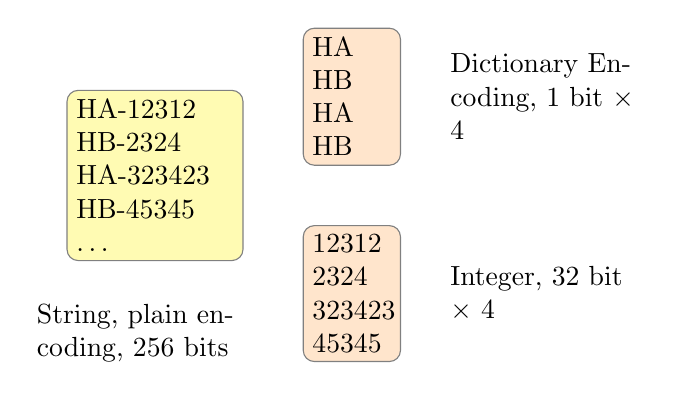
\begin{tikzpicture}
\node[rectangle, rounded corners,fill= yellow!30,draw =gray,text
width = 2cm]at (0,0) {HA-12312\\ HB-2324\\ HA-323423\\ HB-45345 \\ \ldots};
\node[text width = 3cm] at(0,-2) {String, plain encoding, 256 bits};
\node[rectangle, rounded corners, fill= orange!20, draw=gray,text
width=1cm] at (2.5cm, 1cm) {HA\ HB\\ HA\\ HB};
\node[text width=2.5cm] at (5cm, 1cm) {Dictionary Encoding, 1 bit $\times$ 4};
\node[rectangle, rounded corners, fill= orange!20, draw=gray, text width=1cm]
at(2.5cm, -1.5cm) {12312 \\ 2324 \\ 323423 \\ 45345};
\node[text width = 2.5cm] at (5cm, -1.5cm) {Integer, 32 bit $\times$ 4};
\end{tikzpicture}
\caption{Discovering Sub-structure From Column}
\label{fig:example}
\end{figure}


LSTM model with attention has been widely used in sequence-to-sequence
translation. In \cite{grammar_2014}, the authors build a LSTM model to infer grammar
structure from sentences. Inspired by this work, we want to use LSTM with
attention model to infer pattern from column data.

\section{Dataset and Evaluation}
We have collected a dataset consisting of raw data columns. We prepare
the training dataset by applying existing pattern extractors like
PADS\cite{pads_2008} to data columns.

\section{Methods}

Our method is similar to what is described in \cite{grammar_2014}. By flattening
the tree-like pattern to sequencial structure, we are able to directly apply the
LSTM-with-attention model to it. For a given data columns, we will generate a
pattern for each record in the column and choose the most common one as final result.

\section{Key Experiment}
We evaluate the method by compare its result to the one generated from PADS.
We also plan to manually observe the output and make some analysis. The
following evaluations are taken into consideration:
\begin{enumerate}
  \item Error rate. That is, the number of records that cannot fit into the
  generated pattern.
  \item Encoded size compared to PADS. The encoded size is computed by sum up
  the pattern size and the record size after encoding.
\end{enumerate}

\section{Work Plan}
\begin{tabular}{l|l}
May 9th - May 16th & Prepare Dataset\\
\hline
May 17th - May 23rd & Develop the Algorithm and Train on Dataset\\
\hline
May 24th - May 31st & Experiment and Evaluation \\
\hline
Jun 1st - Jun 6th & Writing Report
\end{tabular}

\bibliographystyle{plain}
\bibliography{reference}
\end{document}

